\documentclass[../physical_computing.tex]{subfiles}

\begin{document}

\chapter{Lab Exercise 5 - Using XADC}
\label{sec:appendix_6}

In todays lab we will use one of the IP modules built in to Vivado. Like many chips, the Artix7 FPGA has 
some built in capability for analog to digital conversion. This is intended to read out analog signals used
as diagnostics for the chip. The two quantities usually probed by the ADCs are the temperature of the chip
and the voltages at the supply rails. However, if we choose to we can route the ADC inputs to external ports
of the BASYS3 board and use them to measure external signals. You will have noticed the four 12-way connectors, 
two mounted no each end of the board. These are called PMOD (peripheral module) connectors. Digilent make many
peripherals for the PMOD standard; the DAC card that I supplied with the BASYS3 is one of them. However, one 
of these PMOD connectors can also be used to input signals onto the inbuilt ADC. The connector is labelled
JXADC and it is to the left of the four digit display. 

When using the JXADC port for analog input, the wiring is as follows. The four pins (in two pairs) nearest
to the JXADC label, labelled with `3V3' and `GND' are supply rails used to power expansion connectors. The 
other 8 pins can be thought of four banks of two pins each, arranged on the connector in four vertical pairs.
For the purposes of analog input, the upper of this pair is the $+$ input and the lower one is the $-$ input.

Analog signals come in different varieties. In physics labs, most cables carrying signals are so-called BNC
coaxial cables. These are the black lab cables you connect to oscilloscopes, usually they have RG58 written on
the side, which is a class of cable having standard characteristics. 
Signals on such cables are single ended, which means that the inner conductor at the core of the
coax carries the signal, and the outer conductor which forms a braided sheath around it is connected to ground.
Typically the inner conductor can carry a voltage which is either at a positive or negative voltage with respect
to the outer grounded conductor. Coaxial RG58 cables of the type found in physics labs can carry signals at high
frequencies, up to a few $\rm GHz$ and are very mechanically robust.

It is also quite common to have differential signals. Here
again you have two conductors, but instead of one of them being connected to ground, they are both floating, and
referred to as the $+$ (non-inverting) and $-$ (inverting) input. The signal is the difference in voltage
$V_+-V_-$. Ideally the non-inverting input and the inverting input would always be carrying equal magnitude but 
opposite sign voltages. The common mode voltage, which is the average of the two voltages would be zero. If you 
want really low noise, you then twist the two signal carrying conductors together and surround them with a
grounded sheath. This way of carrying signals is called twisted pair and ground. The advantage of this arrangement
is that it keeps common mode signals to a minimum, and the grounded sheath can have a break in it which breaks
any circuit that may be created in the ground path between two connected instruments. 

In low cost digital circuits, such as on the BASYS3 board, there is rarely any negative voltage rail, and so 
it is not possible to have a negative voltage read out on the board. So, the XADC inputs have two possible modes,
single ended and differential. In single ended mode, you need to connect the lower '-' input of the pair carrying
the signal to GND. The upper input carries the signal. To be read out correctly, this voltage must be positive. 
It cannot be greater than 3.3V because that is the positive voltage rail for the chip, but it may also turn out
later that in reality the voltages that can be read out are between $\rm 0V$ and some other positive voltage
that is lower than $\rm +3.3V$. Between $\rm 0V$ and the full scale voltage, the analog input will be converted to a 12 bit binary unsigned output, where binary zero corresponds to $\rm 0V$ and all ones corresponds to the maximum voltage that can be read out.

You can also configure XADC to read a differential signal but beware - because no negative voltages can be read out, the only way to have a differential signal read is to add a common mode voltage big enough so that the biggest negative voltage anticipated as a signal on either wire, plus the common mode voltage added to both signals, will not be negative. So, for example, suppose you have a differential signal where either the inverting or the non inverting wire can potentially have a voltage of $-0.5\,V$ relative to ground. You then need to add a common mode voltage to both inputs of at least $\rm +0.5V$ relative to ground, otherwise your signal will be distorted by the ADC.

\section{Analog Input, LED Output}
\label{sec:xadcinput}

Start a new Vivado project called xadctoled. Import the usual BASYS3 constraint file. Do not edit the constraint file yet. As usual, specify the \texttt{xc7a35tcpg236-1} device. Click on the link close to the top of the left hand Flow Navigator labelled IP Catalog. A new tab should appear in the large project pane with the top of a very long list of built in IP. Type XADC into the Search box in this pane and select XADC Wizard by double clicking on it. A large IP customisation block appears, shown in Figure \ref{fig:xadcwizard}. The xilinx IP blocks are highly configurable. There are many controls and five tabs to go through. Fortunately we will mostly select the defaults. Set things as follows:

\begin{figure}[htbp]
    \centering
    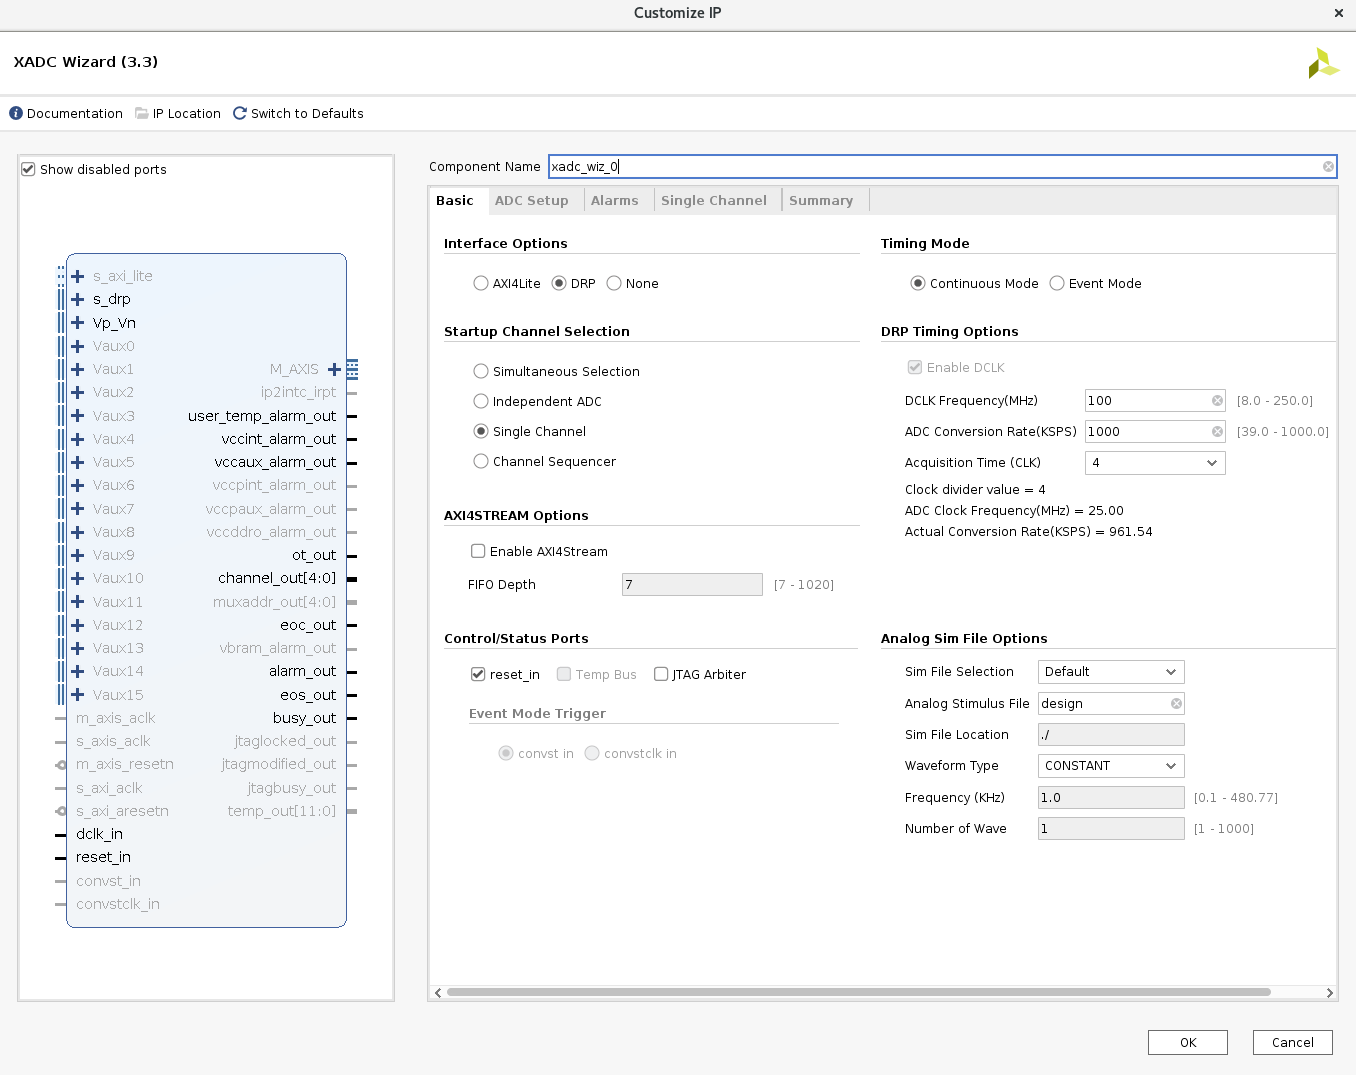
\includegraphics[width=0.7\textwidth]{figures/xadc_wizard.png}
    \caption{The XADC wizard for customising the configuration of the internal 12 bit analog to digital converter.}
    \label{fig:xadcwizard}
\end{figure}

\begin{enumerate}
    \item In the Basic tab, leave everything as it is. Click on the ADC Setup tab.
    \item In the ADC Setup tab, again leave everything as it is. Select the Alarms tab.
    \item In the Alarms tab, we won't be using the XADC to set alarms on overtemperature or supply voltage. 
    You should uncheck all four of the alarms that are on by default. Notice that as you do this, some of the ports on the IP block for XADC become greyed out. Click on the Single Channel tab. 
    \item We will an external pin connected to one of the internal analog to digital converters as the input, so change single channel from its default of TEMPERATURE to one of the options lower down, called \texttt{VAUX14}. Leave everything else alone. Select the Summary tab.
    \item Your summary should read that you have selected the DRP interface, the XADC is operating in single channel mode with the AXI4Stream interface false and continuous timing. The input clock is 100MHz, there is no channel averaging and no external MUX (multiplexing). If all this looks good, click OK in the bottom right hand corner. 
    \item In a window that appears called 'Generate Output Products', accept all the defaults by just clicking Generate. You'll also need to click OK when it announces that it has created an 'out of context run'
    
\end{enumerate}

Next we will connect up the ADC to the LEDs using our own VHDL top level file and the port mapping technique that we used last week. Create a new VHDL file and call it xadctoled.vhd. For ports you will need a clk input and the LED outputs (all 16 of them). You will also need to enable ports L3 and M3, which correspond to the second port along from the lower end of the connector nearest to the switches, enabled and named as follows

\begin{minted}{tcl}
set_property PACKAGE_PIN L3 [get_ports {vauxp14}]				
	set_property IOSTANDARD LVCMOS33 [get_ports {vauxp14}]
set_property PACKAGE_PIN M3 [get_ports {vauxn14}]				
	set_property IOSTANDARD LVCMOS33 [get_ports {vauxn14}]
\end{minted}

In the VHDL source code you will need to make a port map to the \texttt{xadc\_wiz\_0} device. Here is most of the VHDL code you will need.

\begin{minted}{vhdl}
library IEEE;
use IEEE.STD_LOGIC_1164.ALL;

entity xadctoled is
    Port ( clk : in STD_LOGIC;
           led : out STD_LOGIC_VECTOR (15 downto 0);
           vauxp14 : in STD_LOGIC;
           vauxn14 : in STD_LOGIC);
end xadctoled;

architecture Behavioral of xadctoled is
  signal enable, ready: STD_LOGIC;
  signal drpaddress: STD_LOGIC_VECTOR(6 downto 0);
  signal dataread: STD_LOGIC_VECTOR(15 downto 0);
  signal databuffer_d, databuffer_q: STD_LOGIC_VECTOR(15 downto 0);
begin
  process(clk, databuffer_d) begin
    if(clk'event and clk='1') then
      databuffer_q <= databuffer_d;
    end if;
  end process;
  
  -- select data channel
  drpaddress <= "0011110";
  
  -- port map for the ADC
  myadc: entity work.xadc_wiz_0
  port map (
    daddr_in => drpaddress,
    dclk_in => clk,
    den_in => enable,
    di_in => "0000000000000000",
    dwe_in => '0',
    busy_out => open,
    vauxp14 => vauxp14,
    vauxn14 => vauxn14,
    vn_in => '0',
    vp_in => '0',
    alarm_out => open,
    do_out => dataread,
    eoc_out => enable,
    eos_out => open,
    channel_out => open, 
    reset_in => '0',
    drdy_out => ready
    );
    
    -- WARNING: THIS CODE WILL NOT RUN WITHOUT MODIFICATIONS.
    -- here I have left out some code that you will have to
    -- figure out for yourself. First, whenever the ready node
    -- goes to '1', you want to copy the dataread node to the
    -- databuffer defined above in the clk process, but when
    -- ready is '0' you just want that buffer to retain whatever
    -- it was already storing. Secondly, the buffer output needs
    -- to be connected to the LEDs.
    
    end Behavioural;
\end{minted}

Once you have incorporated the above code in your project, you should see the \texttt{adc\_wiz\_0} IP modify to be a subelement of the main xadctoled program. You should also be able to synthesise, implement, and generate your bitstream.

\section{Running XADC}
\label{sec:runningxadc}

To test your ADC, deploy your code on the board. You will need to wire up the 
XADC connector to test it. I suggest that you start by just using a couple of wires to connect the input pins of the ADC directly to the voltage rails. A diagram showing the relevant pins of the JXADC connector, viewed looking in to the connector port, is shown in Figure \ref{fig:jxadc}

\begin{figure}[htbp]
    \centering
    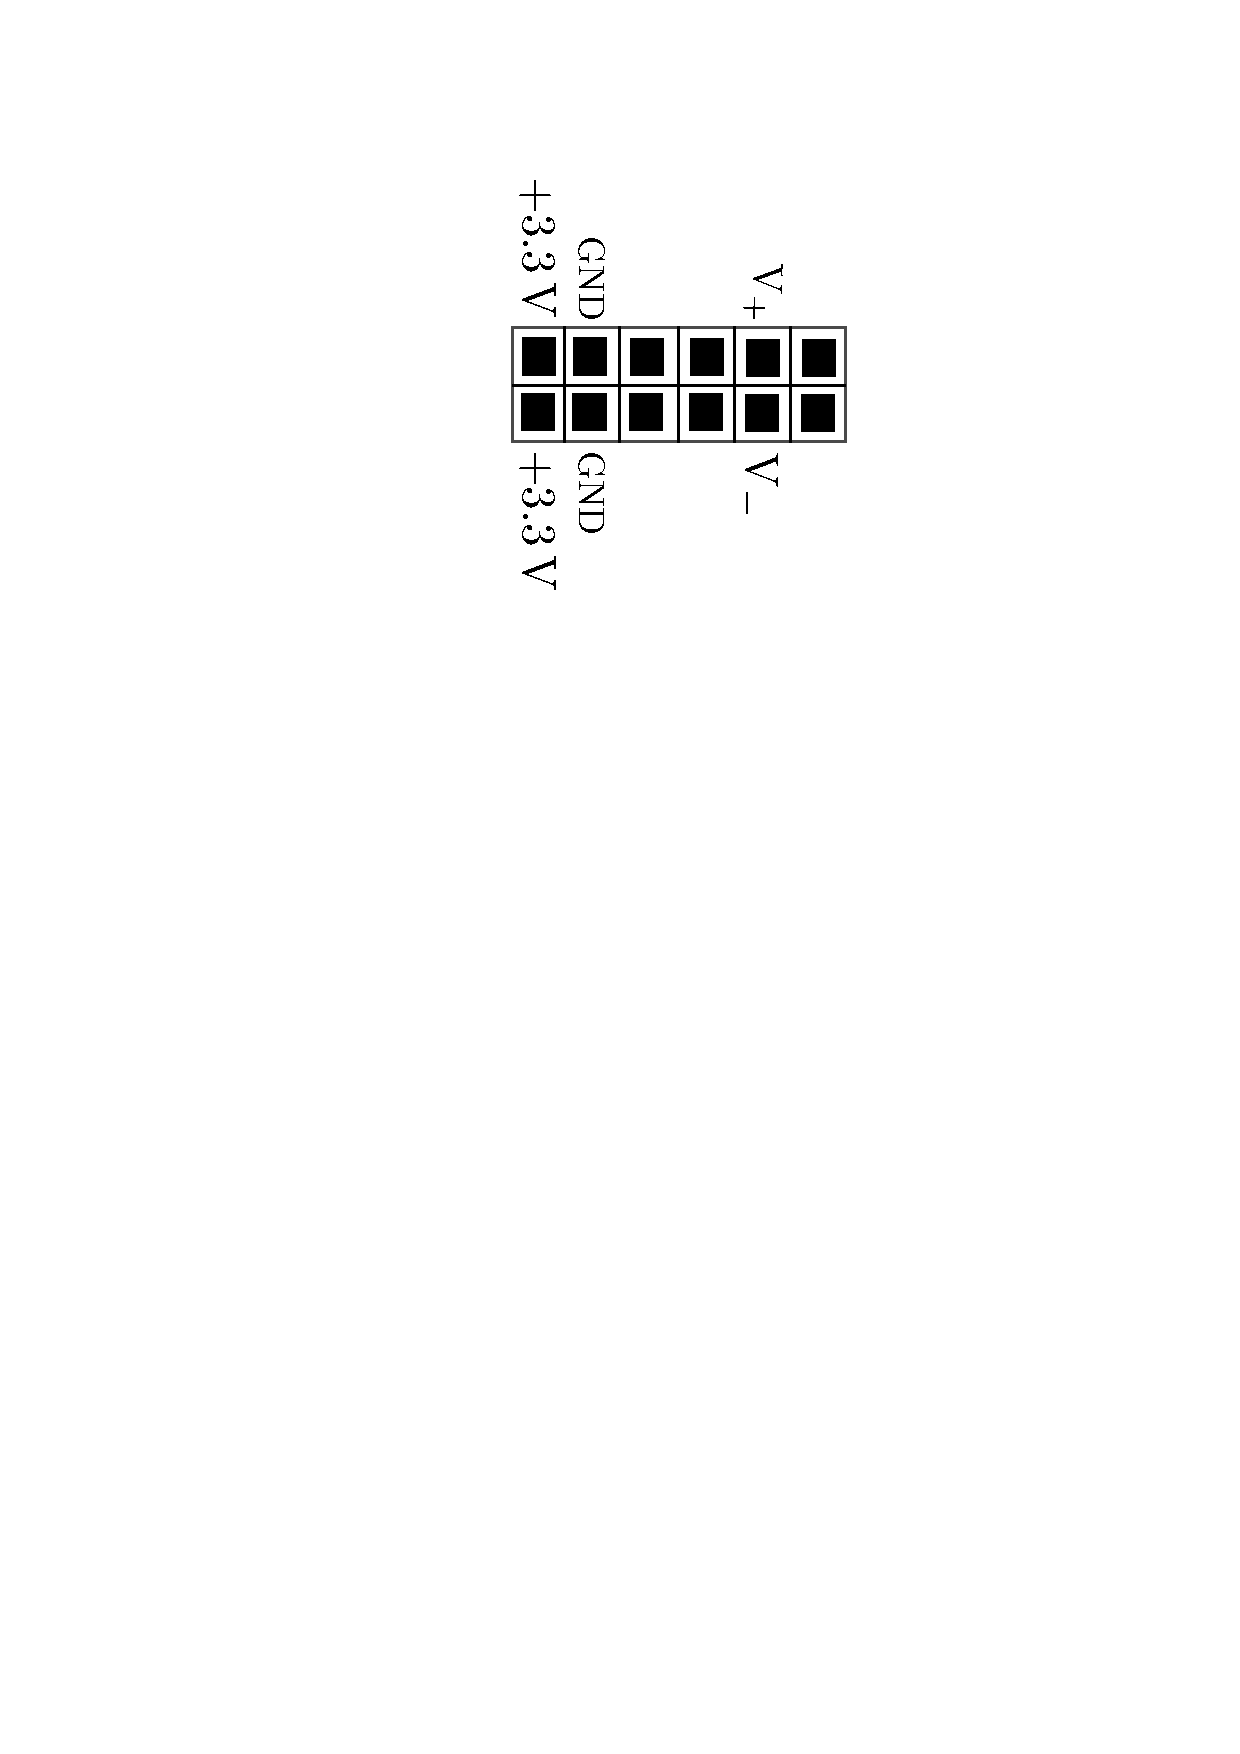
\includegraphics[width=0.3\textwidth]{figures/jxadc.pdf}
    \caption{The pins of the JXADC connector, viewed from the direction looking inwards in to the connector port, showing ground, supply voltage, and the non-inverting and inverting inputs for ADC channel \texttt{VAUX14}.}
    \label{fig:jxadc}
\end{figure}

Connect the $\rm V_-$ terminal to either of the $\rm GND$ terminals with a wire, and connect one end of the other wire to the $\rm V_+$ terminal leaving the other end unconnected for now. Connect the other end of this second wire first to the $\rm GND$ terminal. Now the analogue voltage at both ADC inputs should be $\rm 0V$. However, you should see that about 7 or 8 of the LEDs are lit. The lowest 4 bits are always on because the ADC output is actually only 12 bits, so the four least significant bits are not carrying any information, they are just always high. There are then about 3 or maybe 4 more bits that should be zero, but appear to be lit anyway. This is because these bits are full of noise. ADCs usually have noise in about their lowest three or four bits. They are imperfect devices. Now connect the $\rm V_+$ terminal to $\rm +3.3\,V$ instead. Now all the LEDs should light up. \\

The next experiment is to connect the potentiometer to the ADCs. Do this carefully. Leave $\rm V_-$ connected to $\rm GND$, but remove the lead connected to $\rm V_+$. Connect the two end leads of the potentiometer to $\rm +3.3\,V$ and $\rm GND$, and the middle potentiometer lead to $\rm V_+$. You should now be able to vary the voltage on $V_+$ between $\rm 0V$ and $\rm 3.3V$. What do you see? \\

Using a voltmeter, if you are in the lab, you should be able to measure the voltage on the signal pin of the potentiometer, and determine the voltage at which all the LEDs are first lit. Hint: it's not 3.3V. The full scale deflection of the ADC occurs at a different voltage. \\

\section{A tone generator}
\label{sec:tonegen}

You should all have crystal earpieces. These can be driven directly by a digital output of a BASYS3. In this project you will generate the `A' below middle C, audible through your crystal earpieces. The frequency of this tone, well known to string players because it is traditionally used to tune violins, violas and cellos, is $\rm 440\,Hz$. You therefore need to generate a square wave at this frequency. To do this, calculate how many clock cycles there are in half a period of such a square wave. Make a counter that has enough bits to reach at significantly higher than this number of counts, maybe 4 bits higher. Now, arrange so that when this counter reaches a half period, a \texttt{STD\_LOGIC} register is modified to the \texttt{not} of whatever it was before. The output of this register will therefore go through a full cycle in one period of the wave. By connecting this register output to one of the other PMOD ports (see the constraint file to find a suitable one - the other three PMOD ports are labelled JA, JB and JC), you should be able to connect the crystal earpiece between this port and ground and hear the tone you have made.

\section{A tuneable tone generator}
\label{eq:tuneable}

Now for the clever bit. Make a tone generator whose frequency is controlled by the potentiometer. You have a 12 bit number which you can control with a knob. Make this number control the count that your counter has to reach before resetting, otherwise it's the same as the tone generator project above. You now have made your board convert a signal from analog to digital, and then back from digitial to analog. Tone generators that have a varying pitch with voltage are in fact used quite a lot in diagnostic equipment. For example, in a leak checker, an operator squirts helium gas at some pipework. Rather than having a display that shows the helium level reaching the sensitive detector, the helium level is used to control a variable pitch speaker, so that the operator can focus on squirting the helium in all the right places and just 'hear' when they have found the leak.

\section{Graphical design tool practice}
\label{sec:gui}

The XADC widget can also be used in the graphical designer. Make a new project with an empty graphical design, and add the XADC wizard as IP to the graphical design. Make the same choices of settings as in the port map project. Once you have your XADC design element in the graphical design, you'll need to create your own IP to contain the 16 bit register to store the output, and also wire in the constraints file correctly to connect the external ports. I'm deliberately leaving these instructions vague so that you are challenged to go back to last weeks work and recall how to use the graphical tool. See me or Mitch if you are unsure, though.

\end{document}